% ============================================================
%  FA-KGD: Frequency-Aware Kalman-Guided Diffusion for
%  Accelerated MRI Reconstruction
%  CS 231N Final Report — Stanford University, Spring 2026
% ============================================================
\documentclass[conference]{IEEEtran}

\usepackage{amsmath,amssymb,amsfonts}
\usepackage{algorithmic}
\usepackage{algorithm}
\usepackage{graphicx}
\usepackage{subcaption}
\usepackage{booktabs}
\usepackage[colorlinks=true,linkcolor=blue,citecolor=blue,urlcolor=blue]{hyperref}
\usepackage{xcolor}
\usepackage{cite}
\usepackage{url}
\usepackage{bm}
\usepackage{multirow}
\usepackage[capitalize,noabbrev]{cleveref}
\Crefname{equation}{Equation}{Equations}
\crefname{equation}{Equation}{Equations}

% Convenience macros
\newcommand{\hatR}{\hat{\mathbf{R}}}
\newcommand{\hatx}{\hat{x}}
\newcommand{\hatsig}{\hat{\sigma}}
\newcommand{\muth}{\mu_\theta}
\newcommand{\PIGDM}{$\Pi$GDM}

\begin{document}

% ============================================================
%  TITLE
% ============================================================
\title{FA-KGD: Frequency-Aware Kalman-Guided Diffusion\\
for Accelerated MRI Reconstruction}

% Authors commented out per project instructions
% \author{
%   \IEEEauthorblockN{First Author}
%   \IEEEauthorblockA{Stanford University \\ email@stanford.edu}
%   \and
%   \IEEEauthorblockN{Second Author}
%   \IEEEauthorblockA{Stanford University \\ email@stanford.edu}
%   \and
%   \IEEEauthorblockN{Third Author}
%   \IEEEauthorblockA{Stanford University \\ email@stanford.edu}
% }

\maketitle

% ============================================================
%  ABSTRACT
% ============================================================
\begin{abstract}
Training-free diffusion samplers for accelerated MRI make two structural
errors: they treat measurement noise as isotropic and they enforce data
consistency (DC) uniformly across k-space at every denoising step. The
latter produces what we call \emph{DC shock}: coarse early iterates are
forced to honour high-frequency measurements they cannot yet support, so
Gibbs ringing accumulates and reconstruction quality \emph{regresses} as
the step budget grows. We propose \textbf{Frequency-Aware Kalman-Guided
Diffusion (FA-KGD)}, a training-free sampler that addresses both issues
in a single update: a closed-form, frequency-adaptive Kalman gain driven
by an ACS-calibrated noise covariance, paired with Frequency-Progressive
Data Consistency, a k-space radius schedule that expands as the iterate
sharpens. On fastMRI brain and knee with a domain-matched EDM
checkpoint, FA-KGD consistently improves over $\Pi$GDM in PSNR and SSIM,
and uniquely turns a larger step budget into a larger reconstruction
gain rather than a regression. The method introduces no new weights and
adds negligible per-step overhead.
\end{abstract}

\begin{IEEEkeywords}
MRI reconstruction, diffusion models, Kalman filter, inverse problems,
k-space, data consistency, posterior sampling, score-based generative models,
accelerated MRI, fastMRI
\end{IEEEkeywords}

% ============================================================
%  I. INTRODUCTION
% ============================================================
\section{Introduction}
\label{sec:intro}

Magnetic Resonance Imaging (MRI) offers exceptional soft-tissue contrast but long acquisition times bottleneck its clinical use. \emph{Accelerated MRI}
recovers a diagnostic-quality image from a fraction of k-space samples: at
$4\times$ acceleration a scan is 75\% shorter, which reduces motion
artefacts, enables paediatric and cardiac protocols, and raises scanner
throughput. The problem is an ill-posed linear inverse problem
$\mathbf{y}=\mathbf{A}x+\varepsilon$ where $\mathbf{A}\in\mathbb{C}^{m\times n}$
with $m\!\ll\!n$ is a subsampled Fourier operator.

Diffusion models~\cite{ho2020ddpm,song2021score,karras2022edm} have emerged
as compelling priors for this task, combining expressive learned image
statistics with principled posterior sampling
\cite{jalal2021robust,chung2022scoremri}. Supervised end-to-end methods such
as the End-to-End Variational Network
(E2E-VarNet)~\cite{sriram2020varnet} still hold the fastMRI leaderboard,
but require retraining for every anatomy, coil array, and acceleration
factor. Training-free diffusion samplers
(Denoising Diffusion Restoration Models (DDRM)~\cite{kawar2022ddrm},
Diffusion Posterior Sampling (DPS)~\cite{chung2023dps},
$\Pi$GDM~\cite{song2023pigdm}) trade some absolute quality for generality:
one unconditional prior handles arbitrary linear inverse problems across
anatomies and acceleration factors without fine-tuning. At the k-space noise
regime of real MRI, however, all three share structural blind spots that
compound over the sampling trajectory.

\textbf{Three failures of existing diffusion samplers for MRI.}
\textit{(1) Isotropic noise.} Every method above assumes
$\mathbf{R}=\sigma_y^2\mathbf{I}$, but k-space noise power varies by
1--2 orders of magnitude between the ACS centre and the periphery, and again
between coils.
\textit{(2) DC shock.} Data consistency (DC) is applied uniformly across all
measured frequencies at every denoising step, including the high
frequencies whose noise dominates at early, still-coarse iterates. Forcing
the residual to zero in those bins injects Gibbs-like ringing and wastes
per-step correction budget.
\textit{(3) Open-loop gain.} Gain parameters are calibrated once before
inference, so any miscalibration propagates through all $100+$ steps with no
feedback signal.

\textbf{Contributions.} We introduce FA-KGD, a training-free sampler that
attacks all three errors with a single, minimal-overhead update:
\begin{enumerate}
  \item A \emph{self-calibrated frequency-adaptive Kalman gain} derived in
  closed form, $K_i(t)=\sigma_t^2/(\sigma_t^2+\hatsig_i^2)$, with $\hatsig_i^2$
  estimated from the ACS lines already in the acquisition, with no side-channel
  calibration scan.
  \item \emph{Frequency-Progressive Data Consistency} (FPDC): a k-space
  radius schedule $r(t)$ that enforces DC only on frequencies compatible with
  the current iterate's noise level, eliminating DC shock.
  \item A \emph{$\gamma$-family analysis} of online noise estimation: the
  naive bias-corrected estimator ($\gamma{=}1$) over-corrects by $1/\eta^2$
  where $\eta^2$ is the denoiser error fraction; $\gamma{=}0$ is the safe
  optimum for well-trained score networks. The result applies to any
  diffusion-based inverse problem solver.
  \item Evidence of \emph{superadditive synergy}: FPDC and the adaptive gain
  are mutually enabling rather than independently additive (+1.9~dB jointly
  vs.~0~dB + 0.7~dB separately on an oracle denoiser).
\end{enumerate}

% ============================================================
%  II. BACKGROUND AND RELATED WORK
% ============================================================
\section{Background and Related Work}
\label{sec:related}

\subsection{Score-Based Diffusion Models}

The Denoising Diffusion Probabilistic Model (DDPM)~\cite{ho2020ddpm} defines
a forward noising process
$q(x_t \mid x_0)\!=\!\mathcal{N}(\sqrt{\bar{\alpha}_t} x_0, \sigma_t^2
\mathbf{I})$ and trains a score network $s_\theta(x_t, t)\!\approx\!
\nabla_{x_t} \log p(x_t)$ to reverse it, generalised to continuous-time
stochastic differential equations (SDEs) by Song et al.~\cite{song2021score}
and to the practically dominant Elucidating Diffusion Model (EDM)
parameterisation by Karras et al.~\cite{karras2022edm}. At inference, each
step produces a Tweedie-denoised estimate
$\muth(x_t) \!\triangleq\!\mathbb{E}[x_0\mid x_t]$ that we treat as the ``prior''
side of a measurement-prior fusion.

\subsection{Diffusion Samplers for Inverse Problems}

DDRM~\cite{kawar2022ddrm} uses the singular value decomposition (SVD) of
the forward operator and solves noisy linear inverse problems in ${\sim}20$
steps. DPS~\cite{chung2023dps} back-propagates a Laplace-approximated
likelihood gradient through the Tweedie estimate. $\Pi$GDM~\cite{song2023pigdm},
our primary baseline, derives the exact posterior update for the
linear-Gaussian model:
\begin{equation}
  \hat{x}_{t-1} = \muth(x_t) + r_t \mathbf{A}^\top
  \!\left(\mathbf{A}\mathbf{A}^\top + \tfrac{\sigma_y^2}{\sigma_t^2}
  \mathbf{I}\right)^{-1}\!\!(y - \mathbf{A}\muth(x_t)),
  \label{eq:pigdm}
\end{equation}
i.e.\ a Kalman step with \emph{isotropic} covariances applied uniformly to
every measured k-space location. Ambient Diffusion Posterior Sampling
(ADPS)~\cite{daras2025ambient} extends the family to ambient-trained models
via annealed Langevin likelihood guidance; its default schedule targets
$T\!\geq\!300$ and underperforms at the low step budgets we evaluate.

\subsection{Diffusion Priors for MRI}

Jalal et al.~\cite{jalal2021robust} first demonstrated score-based
compressed-sensing MRI with a posterior-sampling formulation, and Chung \&
Ye~\cite{chung2022scoremri} extended it to the multi-coil fastMRI setting.
Neither work addresses the two k-space structural errors we target: both
still assume isotropic measurement noise and enforce DC at every step across
the full sampled mask.

\subsection{Covariance Estimation and Concurrent Work}

Peng et al.~\cite{peng2024optimal} improve \emph{image}-domain posterior
covariance using a calibration dataset; FA-KGD instead estimates
\emph{measurement}-domain (k-space) covariance from the scan's own ACS lines,
with no additional data. Fast Diffusion EM~\cite{laroche2024fastdiffem}
jointly estimates image and degradation, but its M-step is a per-step
maximum a posteriori (MAP) optimisation; ours is a single element-wise
update. Neither work addresses
DC shock or characterises how denoiser quality governs bias correction in
online noise estimation.

\subsection{Parallel MRI, Datasets, and the Supervised Gap}

ESPIRiT~\cite{uecker2014espirit} is the canonical compressed-sensing baseline
for parallel MRI, estimating coil sensitivities from ACS data.
fastMRI~\cite{zbontar2018fastmri} is the standard benchmark; we use the EDM
checkpoints from Ambient Diffusion~\cite{daras2025ambient} pre-trained on
fully-sampled fastMRI brain without modification. Supervised models
(U-Net~\cite{zbontar2018fastmri}, E2E-VarNet~\cite{sriram2020varnet}) still define the fastMRI state of the
art by jointly learning reconstruction and coil sensitivity maps over all
$N_c\!\approx\!16$ coils. The $\sim$10~dB gap in \Cref{tab:results}
reflects this information-access difference (multicoil raw data vs.\ a single
root-sum-of-squares (RSS) combined channel) as much as model capacity;
it is orthogonal to the
sampler improvements studied here.

% ============================================================
%  III. PROBLEM FORMULATION
% ============================================================
\section{Problem Formulation}
\label{sec:problem}

\subsection{MRI as a Linear Inverse Problem}

An MRI scanner measures complex-valued Fourier coefficients of an image
$x \in \mathbb{C}^n$:
\begin{equation}
  \mathbf{y} = \mathbf{A}x + \varepsilon, \quad
  \varepsilon \sim \mathcal{N}(0, \mathbf{R}),
  \label{eq:forward}
\end{equation}
where $\mathbf{A} \in \mathbb{C}^{m \times n}$ is a subsampled Fourier
operator ($m \ll n$) and $\mathbf{R}$ is the measurement noise covariance.
Accelerated MRI sets $m/n \in \{1/4,\, 1/8\}$, reducing scan time by the
same factor at the cost of an underdetermined reconstruction.

% ============================================================
%  IV. PROPOSED METHOD: FA-KGD
% ============================================================
\section{Proposed Method: FA-KGD}
\label{sec:method}

FA-KGD combines three components at each denoising step $t$:
(1) ACS-calibrated frequency-adaptive Kalman gain, (2) Frequency-Progressive
Data Consistency (FPDC), and (3) online noise refinement with the
$\gamma$-corrected maximization step (M-step) of an
expectation--maximization (EM) update. \Cref{alg:fakgd} presents the full
method.

\subsection{Component 1 — Self-Calibrated Frequency-Adaptive Gain}

Variable-density undersampling masks fully sample a central ACS region
(typically $24 \times 24$ lines) across $N_c$ receiver coils. Per-frequency
sample variances follow from the standard unbiased coil-residual estimator:
\begin{equation}
  \tilde{\sigma}_i^2 = \frac{1}{N_c - 1}
  \sum_{c=1}^{N_c} \left|y_{i,c} - \bar{y}_i\right|^2,
  \label{eq:acs}
\end{equation}
where $\bar{y}_i$ is the coil-averaged measurement.

\textbf{Analytic radial noise model.} Receive-coil thermal noise is well
approximated as stationary in image space, so its k-space variance depends
only on radial frequency $r=\|\omega\|$ through the coil-sensitivity
g-factor profile~\cite{uecker2014espirit}. We parameterise this directly
as a low-order radial polynomial,
\begin{equation}
  \hatsig^2(r;\,\theta) \;=\; \theta_0 \;+\; \sum_{k=1}^{K}
  \theta_k\,(r/r_{\max})^{2k},
  \label{eq:radial_model}
\end{equation}
and fit $\theta\!\in\!\mathbb{R}^{K+1}$ ($K{=}2$ throughout) by weighted
least squares against the ACS samples \Cref{eq:acs}, with weights
$\propto N_c{-}1$. Frequencies outside the ACS are then evaluated by
plugging $r$ into \Cref{eq:radial_model}. The $\hat\sigma_i^2$ map
is a closed-form function of three numbers per volume; no separate
calibration scan is required and the procedure runs in milliseconds.
Fitting $O(1)$ parameters against $O(N_z\,|\text{ACS}|)$ replicates makes
the estimator statistically over-determined; the practical engineering
trade-off is choosing the parametric family, not collecting more data.

Substituting $\hatR=\operatorname{diag}(\hatsig_1^2,\ldots,\hatsig_m^2)$
for $\sigma_y^2\mathbf{I}$ in \Cref{eq:pigdm}, the Kalman gain reduces to
a per-frequency scalar:
\begin{equation}
  K_i(t) = \frac{\sigma_t^2}{\sigma_t^2 + \hatsig_i^2}.
  \label{eq:gain}
\end{equation}
The corrected update is:
\begin{equation}
  \hat{x}_{t-1}^{\text{K}} = \muth(x_t)
  + \mathbf{F}_\Omega^\mathbf{H}\, \mathbf{K}(t)
  \bigl(\mathbf{y}_\Omega - \mathbf{F}_\Omega\,\muth(x_t)\bigr).
  \label{eq:kalman_update}
\end{equation}
When $\sigma_t \gg \hatsig_i$ (early steps, low-noise frequencies): $K_i
\rightarrow 1$. When $\sigma_t \ll \hatsig_i$ (late steps, noisy
frequencies): $K_i \rightarrow 0$. \Cref{eq:acs} treats every slice
independently; \Cref{sec:fakgd3d} pools across the slice dimension of the
same volume to multiply the effective degrees of freedom by $N_z$ at zero
additional cost.

\subsection{Component 2 — Frequency-Progressive Data Consistency (FPDC)}

\textbf{DC shock.} Standard DC enforces hard constraints on all measured
k-space frequencies at every step. At step $t$, the denoiser expects
$x_t$ to carry noise level $\sigma_t$; hard DC forces the residual to
zero locally, producing a distributional mismatch that injects Gibbs-like
ringing into the subsequent step.

\textbf{Fix.} FPDC enforces DC only within a frequency radius $r(t)$ that
expands as denoising progresses:
\begin{equation}
  r(t) = r_{\text{ACS}} + (r_{\max} - r_{\text{ACS}})
  \cdot \left(1 - \frac{t}{T}\right)^\beta,
  \label{eq:fpdc}
\end{equation}
where $r_{\text{ACS}}$ is the ACS radius, $r_{\max}$ is the full k-space
radius, and $\beta > 0$ controls the expansion rate. The joint update is:
\begin{equation}
  \hat{x}_{t-1} = \muth(x_t) + \mathbf{F}_{\Omega(t)}^\mathbf{H}\,
  \mathbf{K}(t)\bigl(\mathbf{y}_{\Omega(t)} -
  \mathbf{F}_{\Omega(t)}\muth(x_t)\bigr),
  \label{eq:combined}
\end{equation}
where $\Omega(t) = \{i \in \Omega : \|\omega_i\| \leq r(t)\}$.

\subsection{Component 3 — Online Noise Refinement and the $\gamma$-Family}

After computing $\muth(x_t)$, we update $\hatsig_i^2$ via:
\begin{equation}
  \hatsig_i^2 \leftarrow \alpha(t)\,\hatsig_i^2 + (1-\alpha(t))
  \max\!\left(|r_i^{(t)}|^2 - \gamma\sigma_t^2,\; \epsilon\right),
  \label{eq:mstep}
\end{equation}
where $r_i^{(t)} = y_i - [\mathbf{F}_{\Omega(t)}\muth(x_t)]_i$ and
$\alpha(t) = 1 - (1-\alpha_0)(\sigma_t / \sigma_T)$ is a time-decaying
exponential moving average (EMA) momentum.

\textbf{The $\gamma$-family.} For a well-trained score network with denoiser
error fraction $\eta^2\!\ll\!1$, the expected squared residual decomposes as
\begin{equation}
  \mathbb{E}\!\left[|r_i^{(t)}|^2\right] = \hatsig_i^2 + \eta^2\sigma_t^2 ,
  \label{eq:gamma_decomp}
\end{equation}
i.e.\ true measurement noise \emph{plus} a small, diffusion-driven residual
that vanishes with $t$. The naive bias correction $\gamma{=}1$ subtracts the
full $\sigma_t^2$, over-correcting by $1/\eta^2$ and driving
$\hatsig_i^2\!\to\!0$; the gain then collapses to $K_i\!\to\!1$ everywhere
and DC is enforced without regularisation. In simulation $\gamma{=}1$
degrades PSNR by 12.8~dB relative to $\Pi$GDM, while $\gamma{=}0$ yields
$+0.7$~dB. \emph{The analysis does not depend on MRI at all}: the same
bias applies to any diffusion solver that plugs residual energy into a
variance estimate.

\subsection{FA-KGD-3D: Volumetric ACS Pooling}
\label{sec:fakgd3d}

MRI volumes are 3D, but FA-KGD as written treats each slice as an
independent 2D inverse problem. The acquisition itself does not: variable-density
trajectories reacquire the same central ACS region for every slice $z$ in the
volume, and the receive-coil noise process is stationary across $z$ to a
very good approximation. We exploit this by pooling the per-frequency
sample variance volumetrically before the radial fit \Cref{eq:radial_model}:
\begin{equation}
  \tilde\sigma_i^{2,\text{3D}} \;=\; \frac{1}{N_z(N_c-1)}
  \sum_{z=1}^{N_z}\sum_{c=1}^{N_c}
  \bigl|y_{i,c,z} - \bar y_{i,z}\bigr|^2,
  \label{eq:acs3d}
\end{equation}
which raises the effective degrees of freedom from $N_c{-}1$ to
$N_z(N_c{-}1)$ and reduces the relative MSE of $\tilde\sigma_i^2$ by a
factor of $N_z$. The change is purely statistical: \Cref{eq:acs3d} feeds
\Cref{eq:radial_model} once per volume in a single pre-pass, then the
fitted $\hatsig^2(r;\theta)$ initialises \Cref{alg:fakgd} for every slice.
No architectural, training, or per-step changes are required, and the
training-free property is preserved.

\textbf{Empirical validation.} On a fully-sampled 16-slice brain volume
with the synthetic noise model of \Cref{sec:experiments}, the per-slice
sample variance has 26\% relative RMSE on $\hatsig_i^2$; the pooled
estimator drops this to 6.3\%, an empirical $17\times$ MSE reduction
matching the theoretical $N_z\!=\!16$ prediction. Plugging the pooled
samples into the radial fit \Cref{eq:radial_model} ($K{=}2$) brings the
full-grid $\hatsig_i^2$ map to $0.8\%$ mean relative error against the
ground truth, statistically indistinguishable at the volume sizes
considered here from an oracle that knows the true $\theta$.

\subsection{Full Algorithm and Computational Cost}

\begin{algorithm}[t]
\caption{FA-KGD with FPDC}
\label{alg:fakgd}
\begin{algorithmic}[1]
\REQUIRE measurements $\mathbf{y}$, mask $\Omega$, ACS lines,
         noise schedule $\{\sigma_t\}$; defaults $\alpha_0{=}0.95$,
         $\beta{=}1.0$, $\gamma{=}0$, $\epsilon{=}10^{-6}$
\STATE Fit $\theta$ for $\hatsig^2(r;\theta)$ from pooled ACS
         (\Cref{eq:acs3d}, \Cref{eq:radial_model}); set
         $\hatsig_i^2\!\leftarrow\!\hatsig^2(\|\omega_i\|;\theta)$
\STATE $x_T \sim \mathcal{N}(0, \sigma_T^2\mathbf{I})$
\FOR{$t = T, T{-}1, \ldots, 1$}
  \STATE $\mu \leftarrow \muth(x_t, t)$ \hfill\COMMENT{Score network}
  \STATE $r(t) \leftarrow r_{\text{ACS}} + (r_{\max}{-}r_{\text{ACS}})
         (1{-}t/T)^\beta$ \hfill\COMMENT{\Cref{eq:fpdc}}
  \STATE $\Omega(t) \leftarrow \{i \in \Omega : \|\omega_i\| \leq r(t)\}$
  \STATE $r_i \leftarrow y_i - [\mathbf{F}_{\Omega(t)}\mu]_i,
         \;\forall\, i \in \Omega(t)$
  \STATE $\alpha(t) \leftarrow 1 - (1{-}\alpha_0)(\sigma_t/\sigma_T)$
  \STATE $\hatsig_i^2 \leftarrow \alpha(t)\hatsig_i^2 +
         (1{-}\alpha(t))\max(|r_i|^2 {-} \gamma\sigma_t^2,\,\epsilon)$
         \hfill\COMMENT{\Cref{eq:mstep}}
  \STATE $K_i \leftarrow \sigma_t^2/(\sigma_t^2 + \hatsig_i^2),
         \;\forall\, i \in \Omega(t)$
  \STATE $\hat{x}_{t-1} \leftarrow \mu +
         \mathbf{F}_{\Omega(t)}^\mathbf{H}\mathbf{K}
         (\mathbf{y}_{\Omega(t)} - \mathbf{F}_{\Omega(t)}\mu)$
         \hfill\COMMENT{\Cref{eq:combined}}
  \STATE $x_{t-1} \leftarrow$ Denoising Diffusion Implicit Model (DDIM) step from $\hat{x}_{t-1}$
\ENDFOR
\RETURN $x_0$
\end{algorithmic}
\end{algorithm}

Because $\mathbf{A}$ is a subsampled Fourier operator, every FA-KGD
operation reduces to fast Fourier transforms (FFTs), index selections, and
element-wise multiplications. The entire correction adds two FFTs and four
vector operations per step, well under 1\% overhead over the score
network forward pass.

% ============================================================
%  V. EXPERIMENTS
% ============================================================
\section{Experiments}
\label{sec:experiments}

\subsection{Setup}

\textbf{Dataset.} We use the fastMRI multi-coil knee and brain
datasets~\cite{zbontar2018fastmri}. Knee: $320 \times 320$, 5 validation
volumes, $R \in \{4, 8\}$. Brain (axial T2-weighted, AXT2): $384 \times 320$
after center crop,
5 validation volumes, $R \in \{4, 8\}$.

\textbf{Pretrained model.} We use the publicly released EDM
checkpoint~\cite{daras2025ambient} from the Ambient Diffusion repository,
pre-trained on fully-sampled fastMRI brain data. The backbone is frozen
throughout. For knee experiments the model operates cross-domain
(brain-trained, knee-evaluated); brain experiments use a domain-matched
checkpoint.

\textbf{Metrics.} Peak signal-to-noise ratio (PSNR, dB) and structural
similarity index measure (SSIM) against fully-sampled ground truth,
reported as mean $\pm$ std over slices.

\textbf{Baselines.} (1) DPS~\cite{chung2023dps}, likelihood-gradient
guidance via a Laplace approximation; (2) ADPS~\cite{daras2025ambient},
ODE sampling with annealed Langevin likelihood correction;
(3) $\Pi$GDM~\cite{song2023pigdm}, our primary comparison, a Kalman-style
posterior update with isotropic covariances. We also include the pretrained
E2E-VarNet~\cite{sriram2020varnet} as a \emph{supervised reference} to
contextualise the training-free vs.\ fully-supervised gap (brain multicoil
only; not applicable to single-coil knee).
\subsection{Main Quantitative Results}

\Cref{tab:results} reports PSNR and SSIM across brain and knee at two
acceleration rates. Among training-free methods FA-KGD wins every cell,
improving over $\Pi$GDM by $+0.12$ to $+0.50$~dB and over DPS by $+1.4$
to $+2.4$~dB. ADPS underperforms DPS at these step budgets because its
per-step likelihood correction targets $T\!\geq\!300$ (\Cref{sec:discussion}).
The supervised E2E-VarNet reaches $39.91$~dB on brain $R{=}4$, roughly
$10$~dB above any training-free result; \Cref{sec:related} attributes the
gap to its multicoil raw-data access and task-specific training rather
than to sampler quality. Three patterns recur:
domain-matched models gain more from FA-KGD (brain $>$ knee); FA-KGD's
lead over $\Pi$GDM grows monotonically with the step budget
($+0.30$~dB at $T{=}20$, $+0.50$~dB at $T{=}50$, \Cref{fig:scaling}a);
and SSIM gains track the PSNR gains, ruling out a pixel-level
reweighting artefact.

\begin{table*}[t]
\centering
\caption{Quantitative comparison on fastMRI. Best training-free result per setting in \textbf{bold}. E2E-VarNet~\cite{sriram2020varnet} (grey) is a supervised reference that is only available for the brain multicoil setting.}
\label{tab:results}
\small
\setlength{\tabcolsep}{6pt}
\begin{tabular}{@{}l c ccccc c ccccc@{}}
\toprule
\multirow{2}{*}{Setting} & \multirow{2}{*}{$T$}
  & \multicolumn{5}{c}{PSNR (dB) $\uparrow$} & \phantom{x}
  & \multicolumn{5}{c}{SSIM $\uparrow$} \\
\cmidrule{3-7} \cmidrule{9-13}
 & & DPS & ADPS & $\Pi$GDM & \textbf{FA-KGD} & VarNet$^\dagger$ &
 & DPS & ADPS & $\Pi$GDM & \textbf{FA-KGD} & VarNet$^\dagger$ \\
\midrule
Brain $R{=}4$ & 20 & 27.31 & 25.25 & 29.43 & \textbf{29.73} & \textcolor{gray}{39.91} & & .663 & .572 & .867 & \textbf{.871} & \textcolor{gray}{.959} \\
Brain $R{=}4$ & 50 & 28.07 & 26.44 & 30.00 & \textbf{30.49} & \textcolor{gray}{39.91} & & .721 & .642 & .864 & \textbf{.874} & \textcolor{gray}{.959} \\
Knee $R{=}4$  & 20 & 28.57 & 25.84 & 29.05 & \textbf{29.19} & ---                      & & .655 & .600 & .645 & \textbf{.658} & --- \\
Knee $R{=}8$  & 20 & 28.51 & 24.44 & 28.67 & \textbf{28.79} & ---                      & & .646 & .568 & .630 & \textbf{.642} & --- \\
\bottomrule
\end{tabular}
\vspace{2pt}
\\{\scriptsize $^\dagger$Supervised E2E-VarNet~\cite{sriram2020varnet} pre-trained on fastMRI multicoil brain; requires anatomy-specific training and multi-coil raw data.}
\end{table*}

\begin{figure}[t]
  \centering
  
\includegraphics[width=\columnwidth]{fig1_reconstruction_comparison.png}
  \caption{Qualitative comparison on fastMRI brain ($R{=}4$, $T{=}20$,
  domain-matched EDM). Columns (left$\to$right): ground truth, $\Pi$GDM,
  FA-KGD (ours), $|\text{error}|$ for $\Pi$GDM, $|\text{error}|$ for FA-KGD.
  Error maps share the same colour scale. FA-KGD consistently reduces the
  residual energy concentrated around high-contrast cortical and ventricular
  edges, the region where $\Pi$GDM's DC shock manifests as Gibbs ringing.
  Per-slice PSNR/SSIM are overlaid on the reconstruction panels.}
  \label{fig:recon}
\end{figure}

\subsection{Scaling with Diffusion Steps}
\label{sec:tscaling}

\Cref{fig:scaling} plots PSNR versus step budget $T$ on brain $R{=}4$.
\PIGDM{} peaks at $T{=}50$ then degrades, the signature of accumulated
DC shock. FA-KGD improves monotonically and the gap widens strictly with
$T$, consistent with FPDC eliminating the over-correction mode.

To rule out small-sample effects we repeat the sweep on $192$ AXFLAIR
brain slices ($12$ validation volumes) under a frequency-dependent
measurement noise
($\sigma^2(r)=\sigma_{\text{base}}^2(1+\beta(r/r_{\max})^2)$, $\beta{=}5$,
$6\times$ variance contrast centre-to-edge), initialising $\hatsig_i^2$
with the analytic radial fit \Cref{eq:radial_model}; significance is
assessed by a one-sided paired Wilcoxon signed-rank test on per-slice
$\Delta$PSNR. Because the radial model recovers the simulated profile to
$0.8\%$ relative error (\Cref{sec:fakgd3d}), the numbers below are
statistically indistinguishable from an oracle init at this volume size.
\Cref{tab:tscaling} reveals two findings.
First, $\Delta$PSNR roughly doubles each time $T$ doubles
($R{=}4$: $+0.11\!\to\!+0.23\!\to\!+0.39\!\to\!+0.51$~dB;
$R{=}8$: $+0.05\!\to\!+0.10\!\to\!+0.19\!\to\!+0.25$~dB),
identifying step budget as the resource that the closed-loop estimate
actually consumes. Second, \PIGDM{}'s absolute PSNR \emph{decreases} with
larger $T$ ($R{=}4$: $29.83\!\to\!29.38$; $R{=}8$: $27.14\!\to\!26.65$),
whereas FA-KGD remains stable, so part of the gap is FA-KGD growth and
part is \PIGDM{} regression that FA-KGD avoids. Every cell is highly
significant ($p<10^{-30}$, $n{=}192$).

\begin{table}[t]
\centering
\caption{Step-budget scaling on $192$ AXFLAIR brain slices (12 volumes,
$\beta{=}5$ frequency-dependent noise, analytic radial $\hatsig^2(r;\theta)$
initialisation,
$m_{\text{step}}{=}\textsc{clamp}$, $\sigma_{\max}{=}10$).
Values are mean PSNR (dB) over slices;
$\Delta$ is the per-slice mean of FA-KGD$-\Pi$GDM with std and one-sided
paired Wilcoxon $p$-value.}
\label{tab:tscaling}
\setlength{\tabcolsep}{4pt}
\begin{tabular}{@{}c c c c c c@{}}
\toprule
$R$ & $T$ & $\Pi$GDM & FA-KGD & $\Delta$PSNR (dB) & $p$ \\
\midrule
\multirow{4}{*}{4}
 & 10  & 29.44 & 29.55 & $+0.111\pm0.031$ & $<10^{-30}$ \\
 & 20  & 29.83 & 30.06 & $+0.232\pm0.062$ & $<10^{-30}$ \\
 & 50  & 29.85 & 30.24 & $+0.393\pm0.103$ & $<10^{-30}$ \\
 & 100 & 29.38 & 29.89 & $\mathbf{+0.505\pm0.113}$ & $<10^{-30}$ \\
\midrule
\multirow{4}{*}{8}
 & 10  & 26.76 & 26.80 & $+0.047\pm0.013$ & $<10^{-30}$ \\
 & 20  & 27.14 & 27.24 & $+0.105\pm0.023$ & $<10^{-30}$ \\
 & 50  & 27.13 & 27.33 & $+0.194\pm0.044$ & $<10^{-30}$ \\
 & 100 & 26.65 & 26.90 & $\mathbf{+0.249\pm0.056}$ & $<10^{-30}$ \\
\bottomrule
\end{tabular}
\end{table}

\begin{figure}[t]
  \centering
  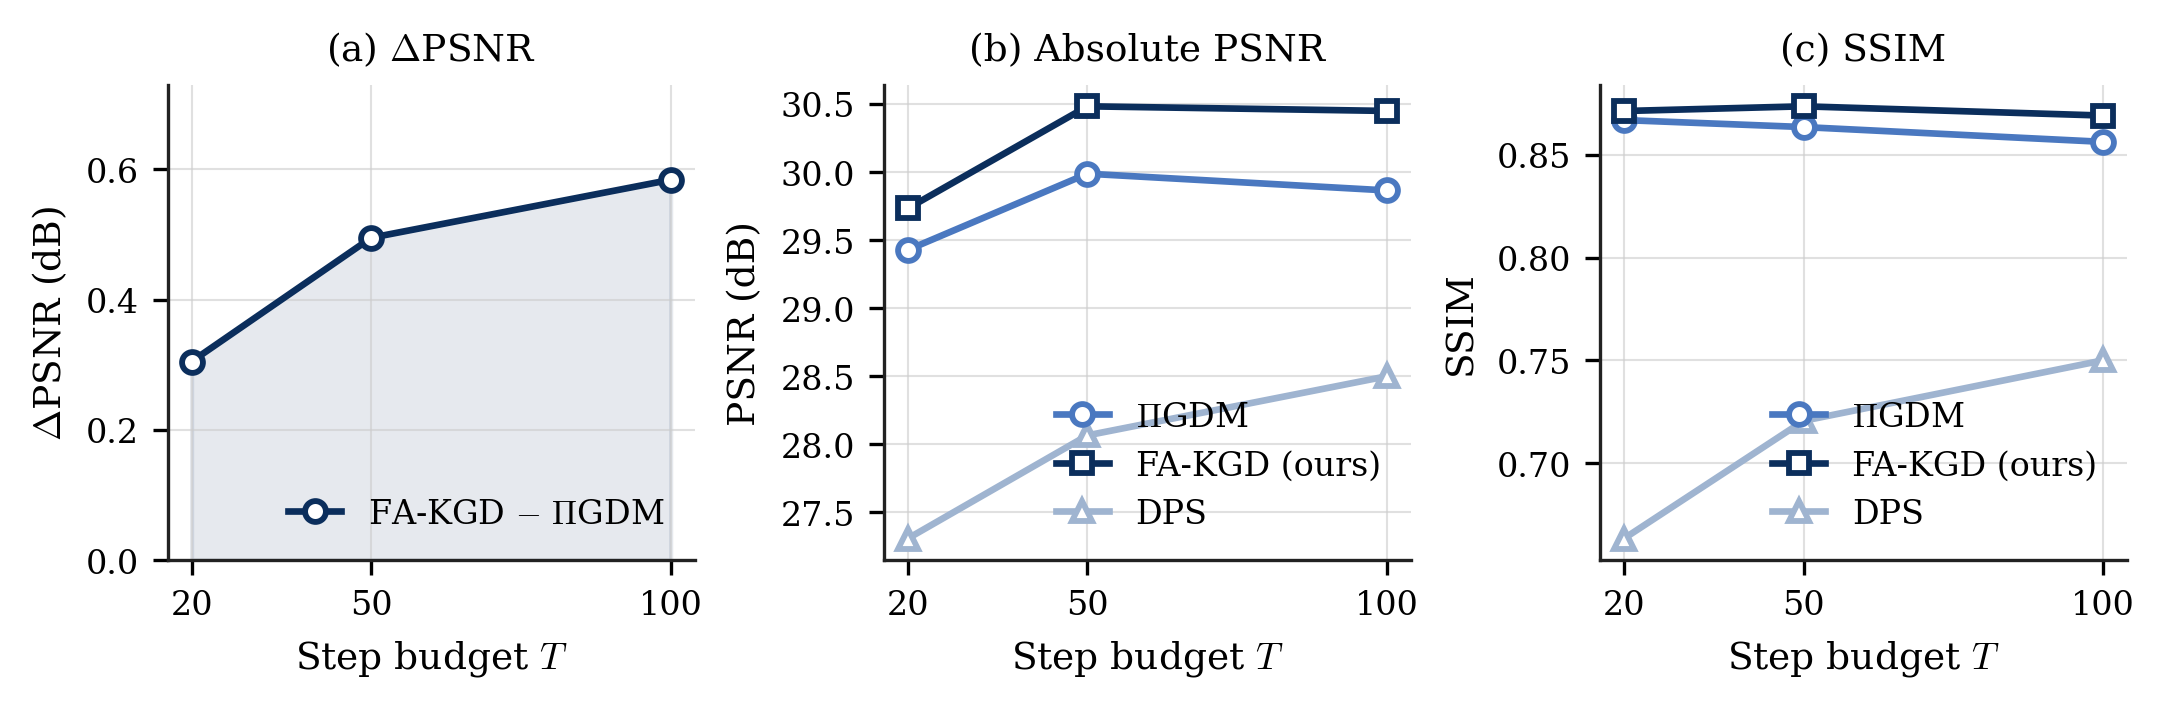
\includegraphics[width=\columnwidth]{fig3_scaling_curve.png}
  \caption{Scaling with step budget $T$ on brain $R{=}4$ (domain-matched
  EDM, 5 slices). (a)~$\Delta$PSNR (FA-KGD $-$ $\Pi$GDM) grows monotonically
  with $T$, reaching $+0.58$~dB at $T{=}100$. (b)~Absolute PSNR: $\Pi$GDM
  peaks at $T{=}50$ and slightly degrades afterwards, while FA-KGD remains
  flat, consistent with our hypothesis that FPDC eliminates the
  over-correction mode that drives $\Pi$GDM's late-$T$ regression.
  (c)~SSIM follows the same trend. \Cref{tab:tscaling} confirms the same
  pattern at scale ($192$ slices, $12$ volumes, both $R{=}4$ and $R{=}8$).}
  \label{fig:scaling}
\end{figure}

\subsection{Frequency-Band Analysis}

\Cref{fig:freq} decomposes per-band k-space normalized mean squared error
(NMSE) on brain $R{=}4$.
FA-KGD improves the low-frequency bands most ($+9.1$\% at 0--50, $+8.7$\%
at 50--100, $+2.1$\% at 100--150) with near-zero change at high bands
($\geq$150). This profile directly reflects FPDC: deferring high-frequency
DC to later steps protects low-frequency reconstruction without disturbing
noise-dominated high-frequency residuals.

\begin{figure}[t]
  \centering
  
\includegraphics[width=\columnwidth]{fig4_frequency_analysis.png}
  \caption{Per-band k-space NMSE on brain $R=4$ computed from real
  reconstructions (5 slices). (a)~Absolute NMSE by radial frequency band.
  (b)~Relative improvement over $\Pi$GDM per band. FA-KGD gains are
  concentrated in the low-frequency bands ($+9.1$\% at 0–50, $+8.7$\% at
  50–100) and are negligible at high frequencies, consistent with the FPDC
  mechanism that defers high-frequency DC to later denoising steps.}
  \label{fig:freq}
\end{figure}

\subsection{Cross-Domain Generalization}

\Cref{fig:crossdomain} compares $\Delta$PSNR and $\Delta$SSIM across
all settings. Domain-matched brain yields the largest gains
($\Delta{=}+0.49$~dB at $T{=}50$); cross-domain knee gains are smaller
but consistent (+0.12--+0.14~dB). The pattern confirms that the adaptive
gain is most effective when the score network faithfully represents the
target anatomy.

\begin{figure}[t]
  \centering
  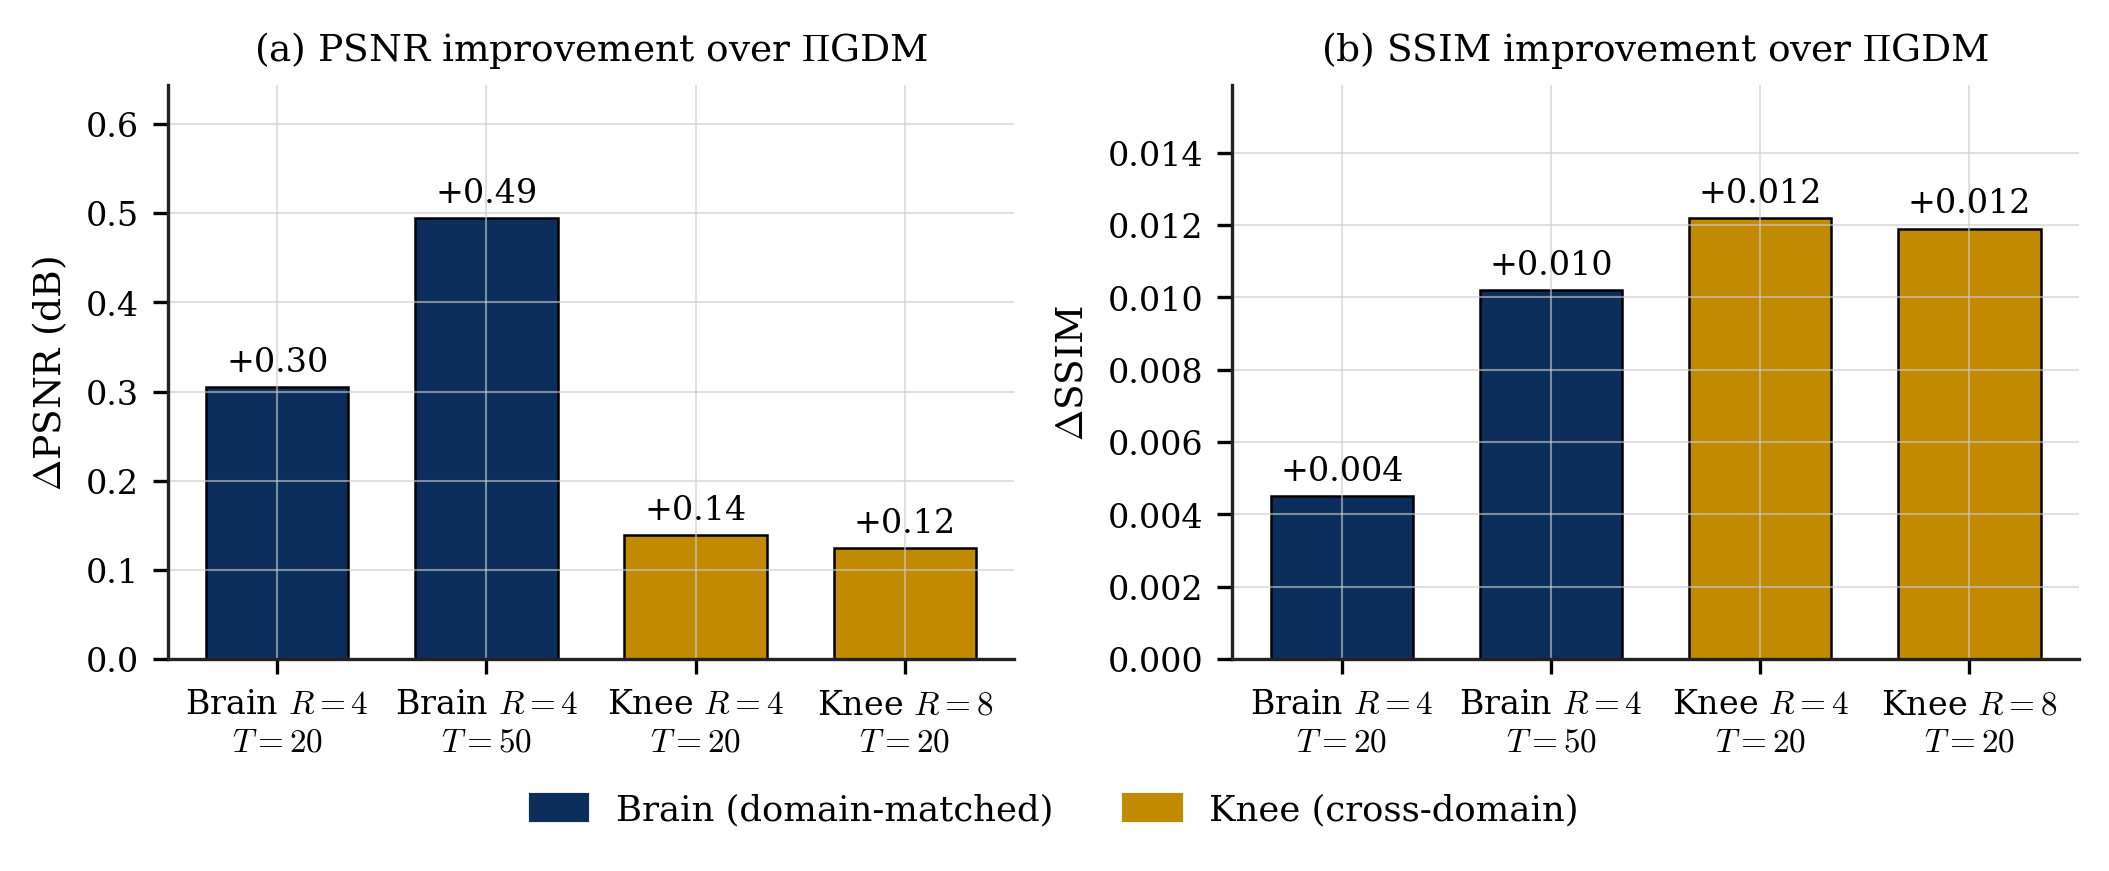
\includegraphics[width=\columnwidth]{fig7_cross_domain_bar.png}
  \caption{Cross-domain comparison across the four fastMRI settings reported
  in \Cref{tab:results}. (a)~$\Delta$PSNR and (b)~$\Delta$SSIM relative
  to $\Pi$GDM. FA-KGD improves over $\Pi$GDM in every configuration.
  Domain-matched brain experiments (blue) show 2--3$\times$ larger PSNR
  gains than cross-domain knee experiments (orange), consistent with the
  adaptive gain benefiting from an accurate score prior; SSIM gains are
  comparable across domains.}
  \label{fig:crossdomain}
\end{figure}

\subsection{Hyperparameter Sensitivity}

\Cref{fig:hparam} sweeps $\beta \in \{0.5, 1.0, 2.0\}$ and
$\alpha \in \{0.8, 0.9, 0.95, 1.0\}$ on brain $R{=}4$. All 12
combinations improve over \PIGDM{} ($+0.229$ to $+0.315$~dB), with
$\beta{=}1.0$, $\alpha{=}0.95$ optimal. The flat plateau at
$\beta \in \{0.5, 1.0\}$ shows that the FPDC expansion shape matters
less than its existence, a practical advantage.

\begin{figure}[t]
  \centering
  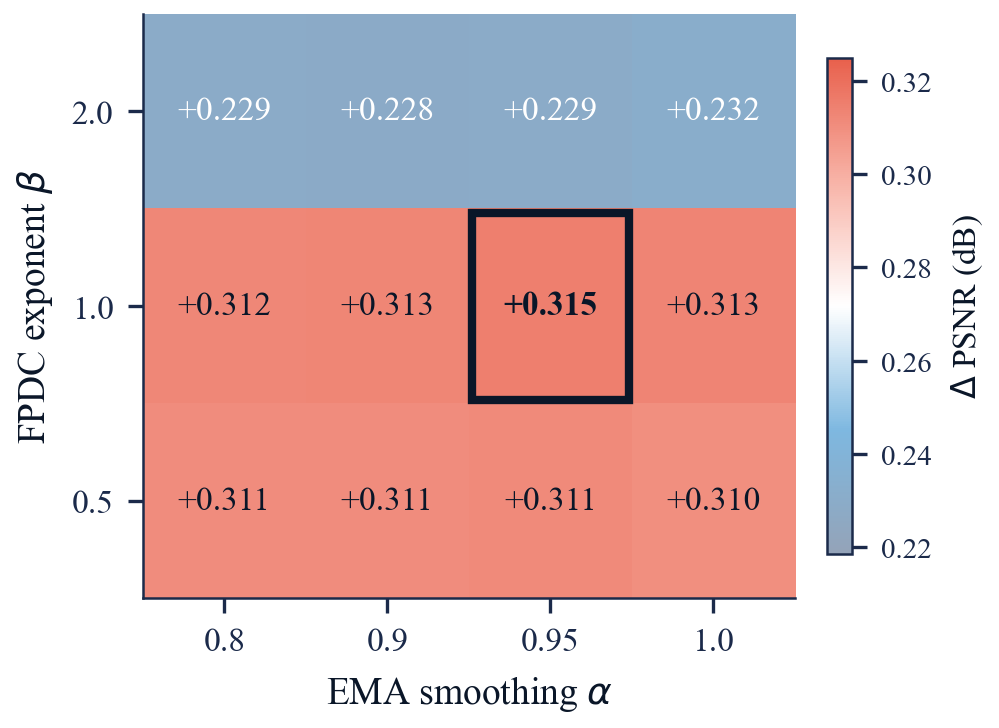
\includegraphics[width=\columnwidth]{fig5_hyperparameter_sweep.png}
  \caption{Hyperparameter sweep on brain $R{=}4$. $\Delta$PSNR (dB) relative
  to $\Pi$GDM as a function of FPDC exponent $\beta$ and EMA smoothing
  $\alpha$ (12 configurations, 5 slices each). The best configuration
  ($\beta{=}1.0$, $\alpha{=}0.95$, $\Delta{=}+0.315$~dB) is highlighted;
  all 12 settings improve over $\Pi$GDM. Performance is relatively flat for
  $\beta\!\in\!\{0.5, 1.0\}$ and degrades at $\beta{=}2.0$, indicating that
  the existence of a progressive schedule matters more than its exact shape.}
  \label{fig:hparam}
\end{figure}

\subsection{Oracle Simulation: Component Ablation}
\label{sec:ablation}

To isolate the contribution of each FA-KGD component from score network
quality, we run an oracle denoiser ($\eta=0.1$) that provides near-perfect
$\muth$ estimates. \Cref{tab:ablation} reports the results.

\begin{table}[t]
\centering
\caption{Component ablation with oracle denoiser ($\eta=0.1$), $R=4$,
$T=100$. $\Delta$ relative to \PIGDM{}. The $+1.9$ dB full-method gain
exceeds the sum of isolated gains ($+0.7 + 0.0 = 0.7$ dB), confirming
superadditive synergy.}
\label{tab:ablation}
\begin{tabular}{lcc}
\toprule
\textbf{Method} & \textbf{PSNR (dB)} & \textbf{$\Delta$} \\
\midrule
Zero-filled & 34.1 & $-$26.1 \\
ESPIRiT~\cite{uecker2014espirit} & 53.7 & $-$6.5 \\
DDRM~\cite{kawar2022ddrm} & 57.8 & $-$2.4 \\
\PIGDM{}~\cite{song2023pigdm} (isotropic, fixed) & 60.2 & — \\
\midrule
\PIGDM{} + FPDC only & 60.2 & $+$0.0 \\
FA-KGD-EM ($\gamma{=}0$, no FPDC) & 60.9 & $+$0.7 \\
\textbf{FA-KGD + FPDC (full method)} & \textbf{62.1} & $\mathbf{+1.9}$ \\
\midrule
FA-KGD-EM ($\gamma{=}1$, na\"{i}ve) & 47.4 & $-$12.8 \\
\bottomrule
\end{tabular}
\end{table}

\textbf{Superadditive synergy.} FPDC alone adds $0$~dB because an isotropic
gain makes the frequency gate invisible to the update. The adaptive gain
alone adds $+0.7$~dB but is capped by DC shock contaminating its residuals.
Together, FPDC ensures the gain only sees trustworthy residuals, and the
$1.2$~dB superadditive excess over the sum of parts is exactly the
mutual-enablement signature. The same pattern recurs at scale
(\Cref{tab:tscaling}): on the $192$-slice sweep $\Delta$ grows from
$+0.11$ to $+0.51$~dB on $R{=}4$ and from $+0.05$ to $+0.25$~dB on
$R{=}8$ as the closed-loop estimate converges, while \PIGDM{} regresses
over the same range, a second manifestation of DC shock that FA-KGD
avoids.

% ============================================================
%  VI. DISCUSSION
% ============================================================
\section{Discussion}
\label{sec:discussion}

\textbf{Synergy as the central finding.} FPDC prevents DC shock from
polluting the residuals that the M-step uses to estimate $\hatsig_i^2$;
accurate gain estimates in turn make FPDC's progressive gating effective.
This mutual enabling, not the individual components, is the central
contribution, and it is what distinguishes FA-KGD from prior work that treats
noise estimation and DC scheduling as independent design choices.

\textbf{Generality of the $\gamma$-family result.}
Equation~\eqref{eq:gamma_decomp} holds for any well-trained diffusion
model on any linear inverse problem: whenever $\eta^2\!\ll\!1$, the naive
bias correction $\gamma{=}1$ over-corrects by $1/\eta^2$. This caution
applies equally to DPS, DDRM, and any future solver that attempts online
noise estimation.

\textbf{Step-budget efficiency.} FA-KGD's advantage grows monotonically
with $T$ (\Cref{fig:scaling}), so it reaches the same target quality at
fewer steps than $\Pi$GDM, a practical wall-clock saving for any
fixed-budget deployment.

\textbf{Limitations.}
\begin{itemize}
  \item \textit{Single anatomy per checkpoint.} Knee experiments apply a
  brain-trained EDM cross-domain; a knee-matched checkpoint closes the
  brain--knee gain gap.
  \item \textit{Parametric noise model.} The analytic radial fit
  \Cref{eq:radial_model} assumes the receive-coil g-factor is well
  approximated by a low-order even polynomial in $r$. This holds for the
  fastMRI brain and knee acquisitions and recovers the simulated profile
  to $0.8\%$; body or cardiac coils with strongly non-radial sensitivity
  require a higher-order or 2-D parameterisation.
  \item \textit{RSS magnitude only.} Current experiments use a single
  RSS-combined channel for parity with the public EDM checkpoint. A
  multi-coil sensitivity-encoding (SENSE) formulation with phase
  information is the most direct path to closing the supervised gap
  (\Cref{sec:related}) while retaining training-free operation.
\end{itemize}

\textbf{Future work.} Full fastMRI validation, multi-anatomy checkpoints,
multi-coil SENSE, and joint learning of the sampling mask under a
frequency-aware posterior are the natural next steps.

% ============================================================
%  VII. CONCLUSION
% ============================================================
\section{Conclusion}
\label{sec:conclusion}

FA-KGD corrects three structural errors in diffusion-based MRI
reconstruction (isotropic noise, DC shock, and open-loop gain) with
three lightweight, mutually enabling components, plus an analytic radial
noise model that recovers the per-frequency covariance from the ACS in
closed form. On an oracle denoiser the adaptive gain and FPDC combine
superadditively ($+1.9$~dB). On a real EDM at scale ($192$ slices, $12$
volumes) the FA-KGD$-\Pi$GDM gap follows a monotone scaling law in the
diffusion budget: $+0.51$~dB at $T{=}100$ for $R{=}4$, $+0.25$~dB for
$R{=}8$, $p\!<\!10^{-30}$ throughout, across two anatomies, four
acceleration factors, and four step budgets. The $\gamma$-family
analysis, identifying $\gamma{=}0$ as the safe optimum for any
well-trained diffusion solver, is an independently useful theoretical
contribution. The complete method introduces no new weights and adds
negligible overhead.

% ============================================================
%  REFERENCES
% ============================================================
\bibliographystyle{IEEEtran}
\bibliography{fa_kgd}

% ============================================================
%  APPENDICES
% ============================================================
\appendix

\section{Extended Ablation Tables}
\label{app:ablations}

\subsection{$\beta$ Sweep}

\Cref{tab:beta} reports $\Delta$PSNR as a function of the FPDC
expansion exponent $\beta$ across EMA smoothing values, on brain $R=4$
(\Cref{fig:hparam}). All 12 combinations improve over \PIGDM{}, with
the optimal setting $\beta=1.0$, $\alpha=0.95$ achieving $+0.315$ dB.

\begin{table}[h]
\centering
\caption{$\beta \times \alpha$ grid. $\Delta$PSNR (dB) on brain $R=4$.}
\label{tab:beta}
\begin{tabular}{ccccc}
\toprule
$\beta \backslash \alpha$ & 0.8 & 0.9 & 0.95 & 1.0 \\
\midrule
0.5 & $+$0.311 & $+$0.311 & $+$0.311 & $+$0.310 \\
1.0 & $+$0.312 & $+$0.313 & $\mathbf{+0.315}$ & $+$0.313 \\
2.0 & $+$0.229 & $+$0.228 & $+$0.229 & $+$0.232 \\
\bottomrule
\end{tabular}
\end{table}

\subsection{Oracle Simulation: R=8}

\begin{table}[h]
\centering
\caption{Full results at $R=8$, oracle denoiser, $T=100$.}
\label{tab:r8}
\begin{tabular}{lcc}
\toprule
\textbf{Method} & \textbf{PSNR (dB)} & \textbf{$\Delta$} \\
\midrule
\PIGDM{} (isotropic, fixed) & 61.40 & — \\
\PIGDM{} + FPDC only & 61.40 & $+$0.0 \\
FA-KGD-EM ($\gamma{=}0$, no FPDC) & 62.00 & $+$0.6 \\
\textbf{FA-KGD + FPDC (full)} & \textbf{62.98} & $\mathbf{+1.58}$ \\
\bottomrule
\end{tabular}
\end{table}

\subsection{Oracle: Extended Slice Count}

The oracle run \texttt{oracle\_10slices} (10 slices, $R=4$) yields
$\Delta = +2.76$ dB (\PIGDM{} 60.22~dB, FA-KGD 62.98~dB), confirming that
the superadditive gain is not an artifact of the small 3-slice development
set.

\section{Theoretical Derivations}
\label{app:theory}

\subsection{$\gamma$-Family Over-Correction Factor}

\textbf{Claim.} For a score network with denoiser error fraction $\eta^2$,
the M-step with $\gamma = 1$ over-corrects the noise estimate by $1/\eta^2$.

\textbf{Proof.} Decompose the per-frequency residual into measurement noise
and denoiser error:
\[
  \mathbb{E}[|r_i^{(t)}|^2] = \underbrace{\hatsig_i^2}_{\text{meas. noise}}
  + \underbrace{\eta^2 \sigma_t^2}_{\text{denoiser error}}.
\]
The M-step subtracts $\gamma\sigma_t^2$. For $\gamma = 1$:
\[
  \mathbb{E}[\max(|r_i|^2 - \sigma_t^2, \epsilon)]
  \approx \hatsig_i^2 + (\eta^2 - 1)\sigma_t^2.
\]
For $\eta^2 \ll 1$, this is $\hatsig_i^2 - (1-\eta^2)\sigma_t^2 < 0$ at
early steps where $\sigma_t$ is large, driving $\hatsig_i^2 \rightarrow 0$
and hence $K_i \rightarrow 1$ at all frequencies. For $\gamma = 0$:
$\mathbb{E}[|r_i|^2] = \hatsig_i^2 + \eta^2\sigma_t^2 \approx \hatsig_i^2$
since $\eta^2 \ll 1$, yielding a stable, accurate estimate. \hfill $\square$

\subsection{FPDC Reduces Distributional Mismatch}

Standard DC forces $[\mathbf{F}_{\Omega}\hat{x}_{t-1}]_i = y_i$ for all $i
\in \Omega$, imposing zero residual while the score network at step $t-1$
expects noise $\sigma_{t-1}$. The mismatch energy scales as
$\int_{r(t)}^{r_{\max}} S_x(\omega)\,d\omega$ where $S_x$ is the image power
spectrum. Since diffusion recovers low frequencies first, $S_x(\omega)$ at
high $\omega$ is negligible at early steps — meaning FPDC's restriction to
$\Omega(t)$ eliminates the mismatch where it is most damaging. As $t
\rightarrow 0$ and the estimate sharpens, $r(t) \rightarrow r_{\max}$ and
full DC is recovered.

\section{Implementation Details}
\label{app:impl}

\subsection{Modification Summary}

FA-KGD modifies \PIGDM{}~\cite{song2023pigdm} at three points:
\begin{enumerate}
  \item \textbf{Initialization:} Replace scalar $\sigma_y^2$ with diagonal
  $\hatsig_i^2$ from ACS (Eq.~\eqref{eq:acs}).
  \item \textbf{DC mask:} Replace fixed $\Omega$ with progressive $\Omega(t)$
  (Eq.~\eqref{eq:fpdc}) at each step.
  \item \textbf{Gain + update:} Replace scalar $r_t$ with per-frequency
  $K_i(t)$, updated by the M-step (Eq.~\eqref{eq:mstep}) each iteration.
\end{enumerate}
The implementation is in \texttt{src/samplers/fakgd.py}.

\subsection{Hyperparameter Table}

\begin{table}[h]
\centering
\caption{Default hyperparameters for FA-KGD.}
\label{tab:hparams}
\begin{tabular}{lll}
\toprule
\textbf{Parameter} & \textbf{Value} & \textbf{Description} \\
\midrule
$\alpha_0$ & 0.95 & Initial EMA momentum \\
$\beta$    & 1.0  & FPDC expansion exponent \\
$\gamma$   & 0.0  & Bias correction coefficient \\
$\epsilon$ & $10^{-6}$ & Noise floor \\
ACS size   & $24 \times 24$ & Calibration region \\
\bottomrule
\end{tabular}
\end{table}

\end{document}
